%%%%%%%%%%%%%%%%%%%%%%%%%%%%%%%%%%%%%%%%%%%%%%%%%%%%%%%%%%%%%%%%%%%%%
%% This is a (brief) model paper using the achemso class
%% The document class accepts keyval options, which should include
%% the target journal and optionally the manuscript type.
%%%%%%%%%%%%%%%%%%%%%%%%%%%%%%%%%%%%%%%%%%%%%%%%%%%%%%%%%%%%%%%%%%%%%
\documentclass[journal=jacsat,manuscript=article]{achemso}

%%%%%%%%%%%%%%%%%%%%%%%%%%%%%%%%%%%%%%%%%%%%%%%%%%%%%%%%%%%%%%%%%%%%%
%% Place any additional packages needed here.  Only include packages
%% which are essential, to avoid problems later.
%%%%%%%%%%%%%%%%%%%%%%%%%%%%%%%%%%%%%%%%%%%%%%%%%%%%%%%%%%%%%%%%%%%%%
\usepackage{multirow}
\usepackage{chemformula} % Formula subscripts using \ch{}
\usepackage[T1]{fontenc} % Use modern font encodings
\usepackage{verbatim}
%% The amssymb package provides various useful mathematical symbols
\usepackage{amssymb}
%% The amsthm package provides extended theorem environments
%% \usepackage{amsthm}

%% The lineno packages adds line numbers. Start line numbering with
%% \begin{linenumbers}, end it with \end{linenumbers}. Or switch it on
%% for the whole article with \linenumbers.
%% \usepackage{lineno}

%\usepackage{graphicx}
%\graphicspath{ {./SI_images/} }

\usepackage{tabularx}

\usepackage{float} 
\usepackage{tikz}
\usepackage{longtable}
\usepackage{bm}
\usepackage{caption}
\usepackage{arydshln}




% for cross reference
\newcommand*\mycommand[1]{\texttt{\emph{#1}}}
\renewcommand{\thefigure}{S\arabic{figure}}
\renewcommand{\thetable}{S\arabic{table}} 
\renewcommand{\thepage}{S\arabic{page}}  

\usepackage[symbol]{footmisc}
\author{Barnabas P. Agbodekhe}
\author{Dinis O. Abranches}
\author{Montana N. Carlozo}
\author{Kyla D. Jones}
\author{Alexander W.~Dowling}
\author{Edward J. Maginn}
\email{ed@nd.edu}
%\phone{+123 (0)123 4445556}
%\fax{+123 (0)123 4445557}
\affiliation[University of Notre Dame]
{Department of Chemical and Biomolecular Engineering, University of Notre Dame, Notre Dame, IN 46556, USA}
%\alsoaffiliation[Second University]{Department of Chemistry, Second University, Nearby Town}


\title{Supporting Information for \\ Integrating Group Contribution Models with Gaussian Process Regression for Simple, Generalizable, and Accurate Thermophysical Property Prediction}

\begin{document}
\newpage

\section{Methods and Data}

\subsection{Data Collection and Preparation}

\subsubsection{Joback and Reid GC Predictions}

\begin{figure}
    \centering
    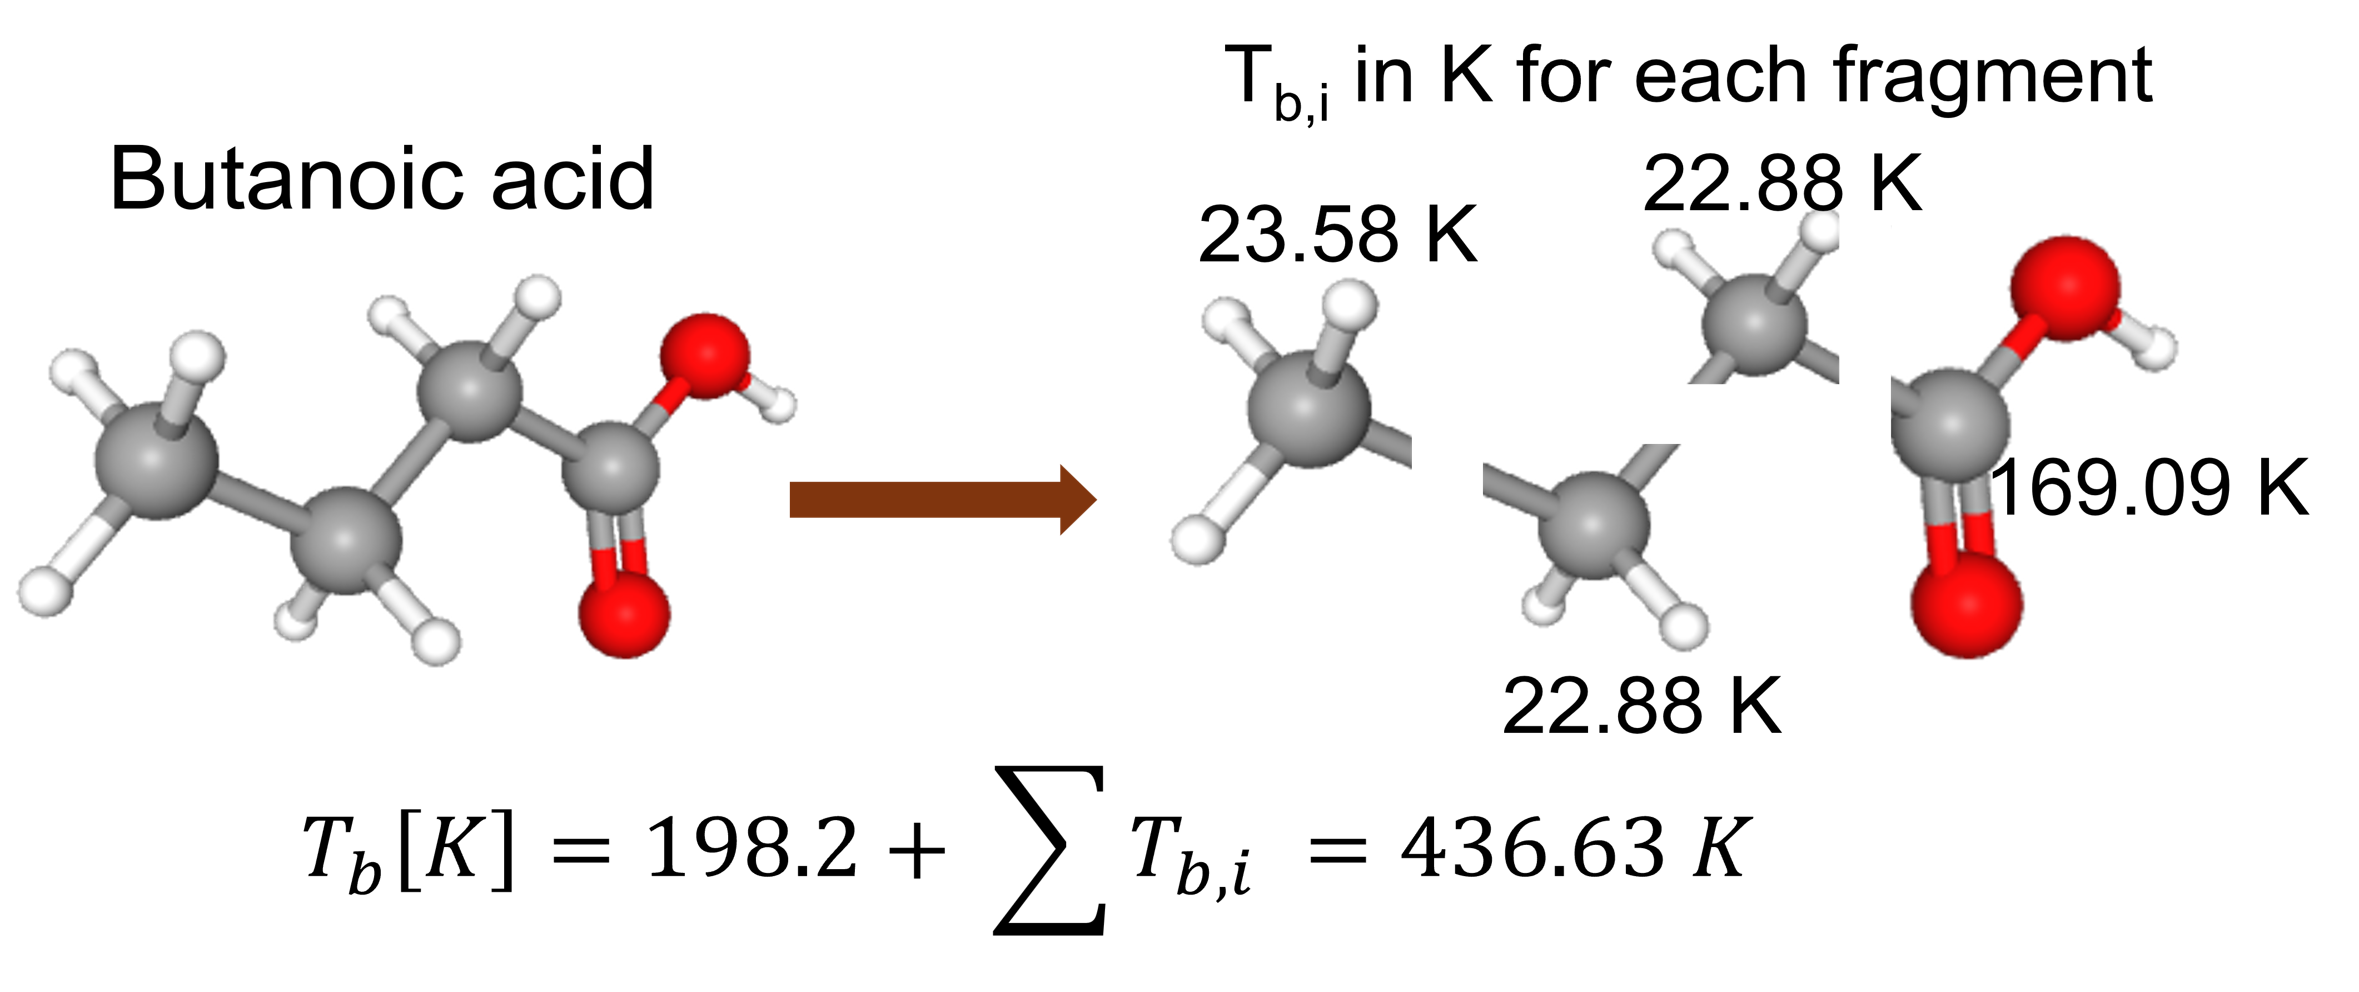
\includegraphics[width=1\linewidth]{images/GC_method_illustration.png}
    \caption{Illustration of Joback and Reid (JR) GC method}
    \label{fig:JR_GC_illustration}
\end{figure}


\subsection{Data Pre-processing}

\subsubsection{Data Quality}

\begin{figure}[H]
    \centering
    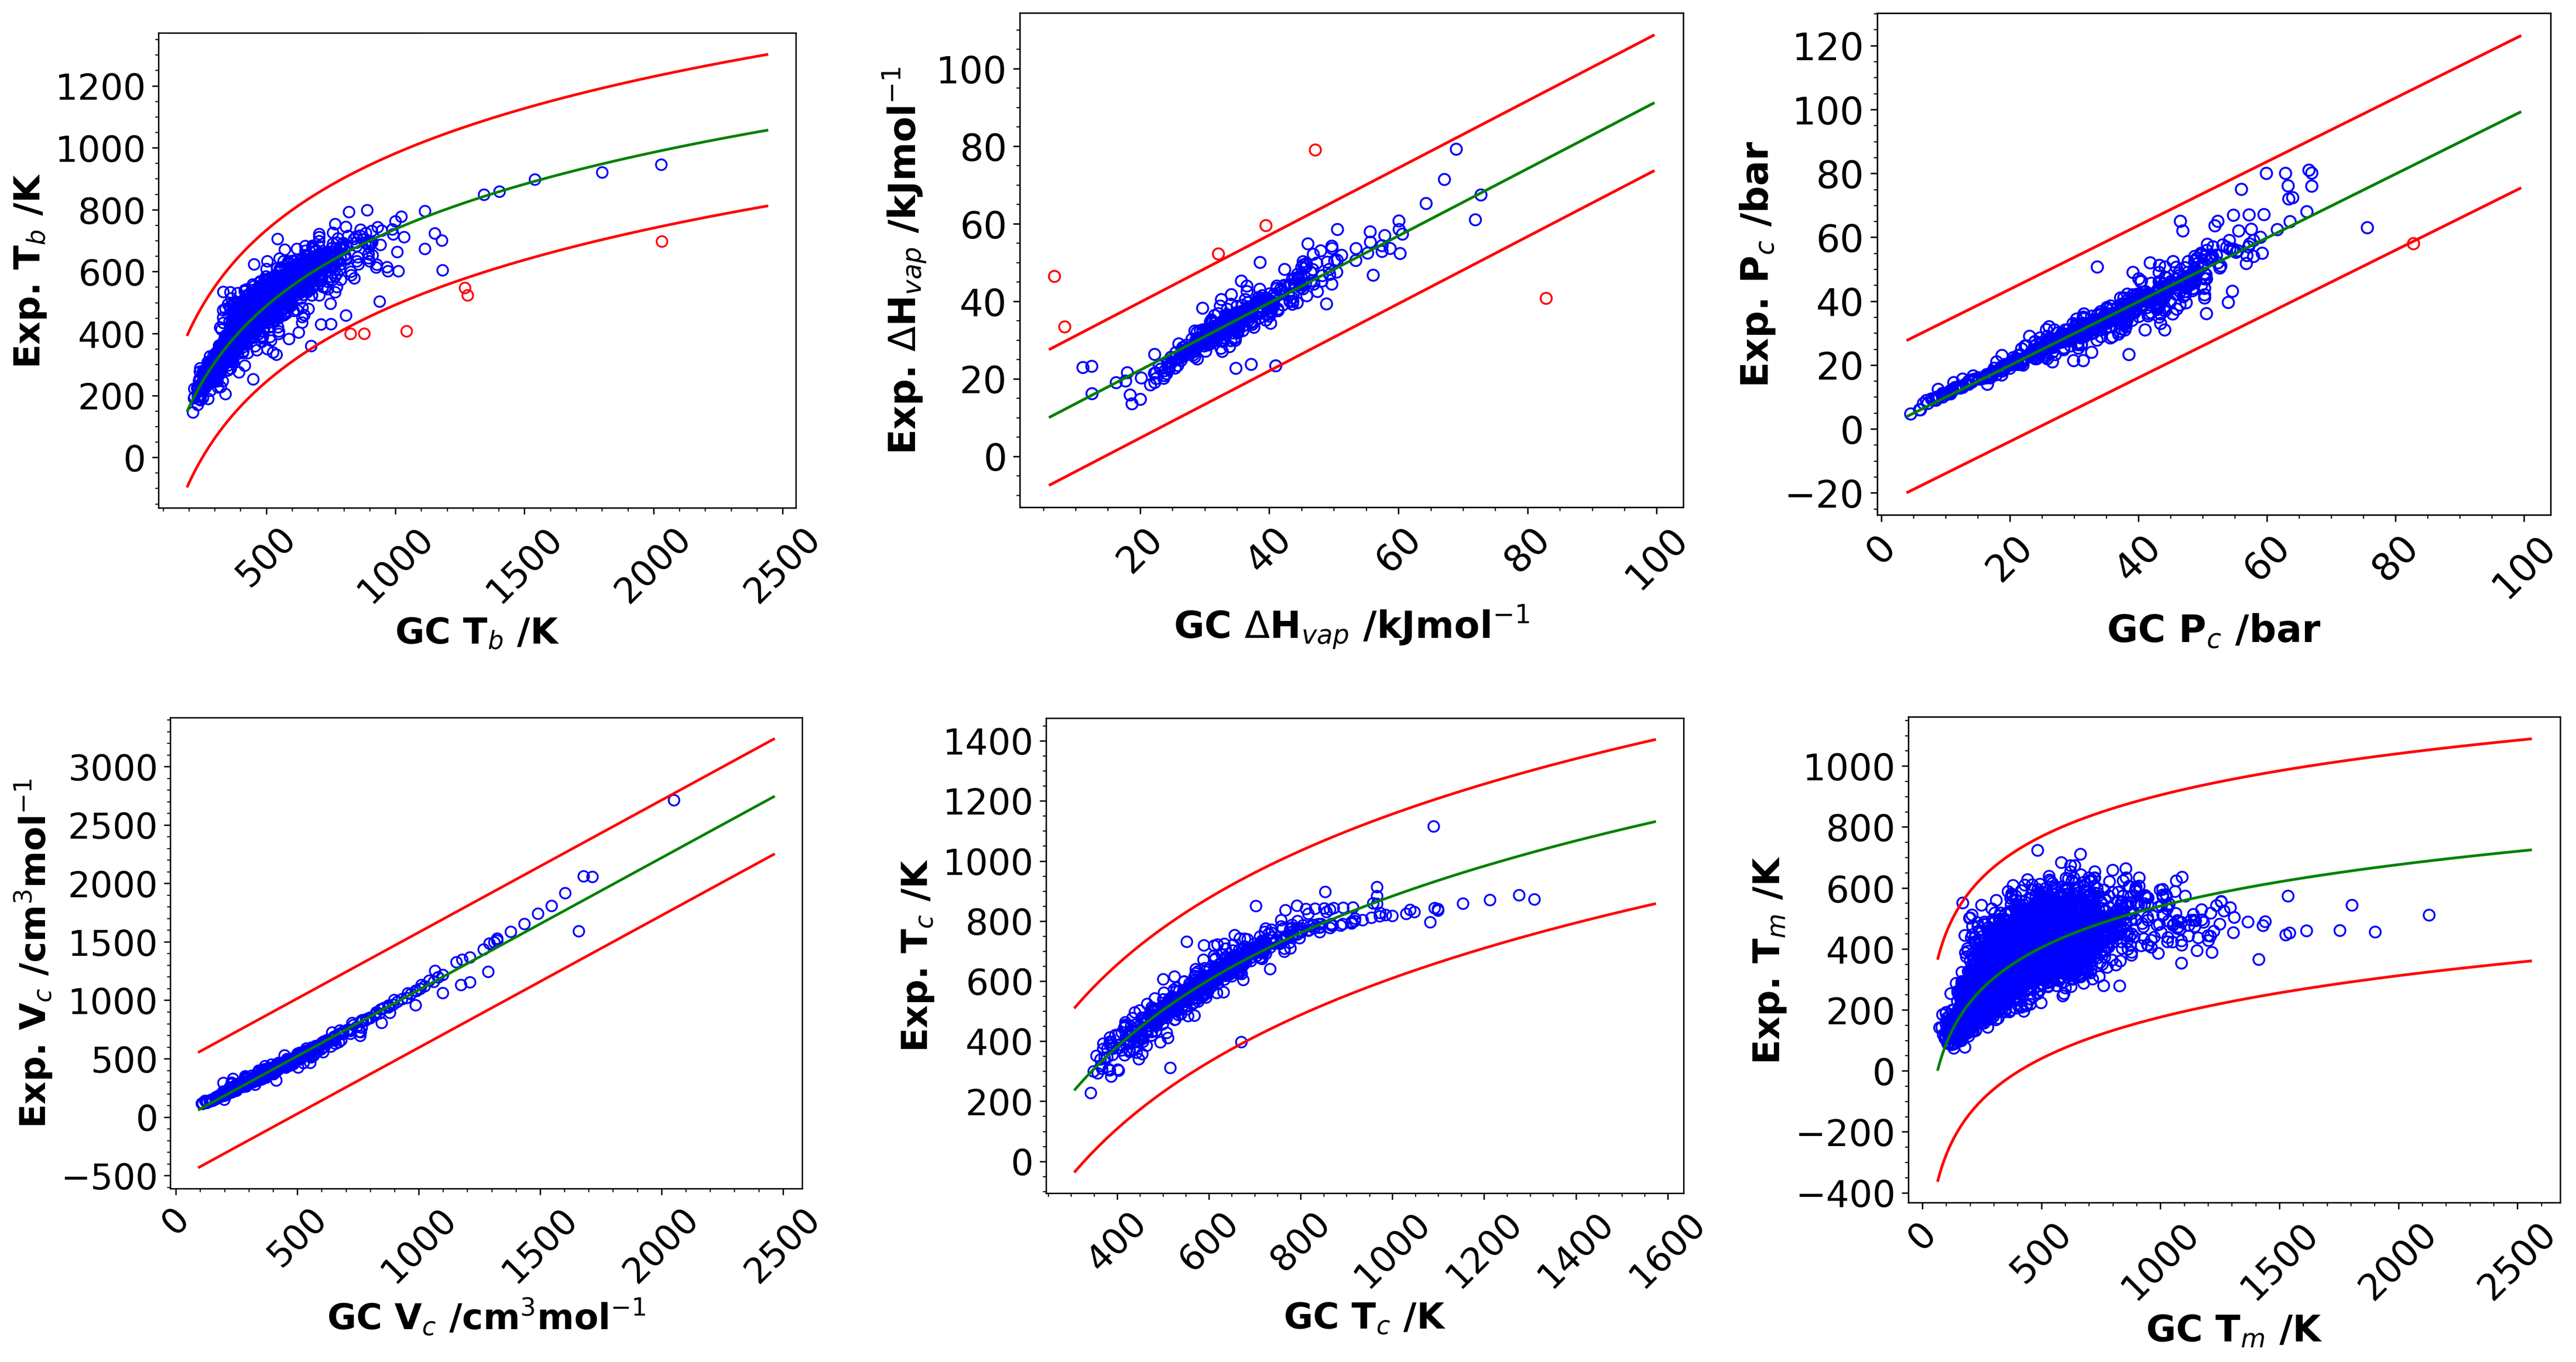
\includegraphics[width=1\linewidth]{images/2D_outlier_analysis.png}
    \caption{Outlier analysis using JR GC predictions}
    \label{fig:2D_outlier_analysis}
\end{figure}



\begin{figure}[H]
    \centering
    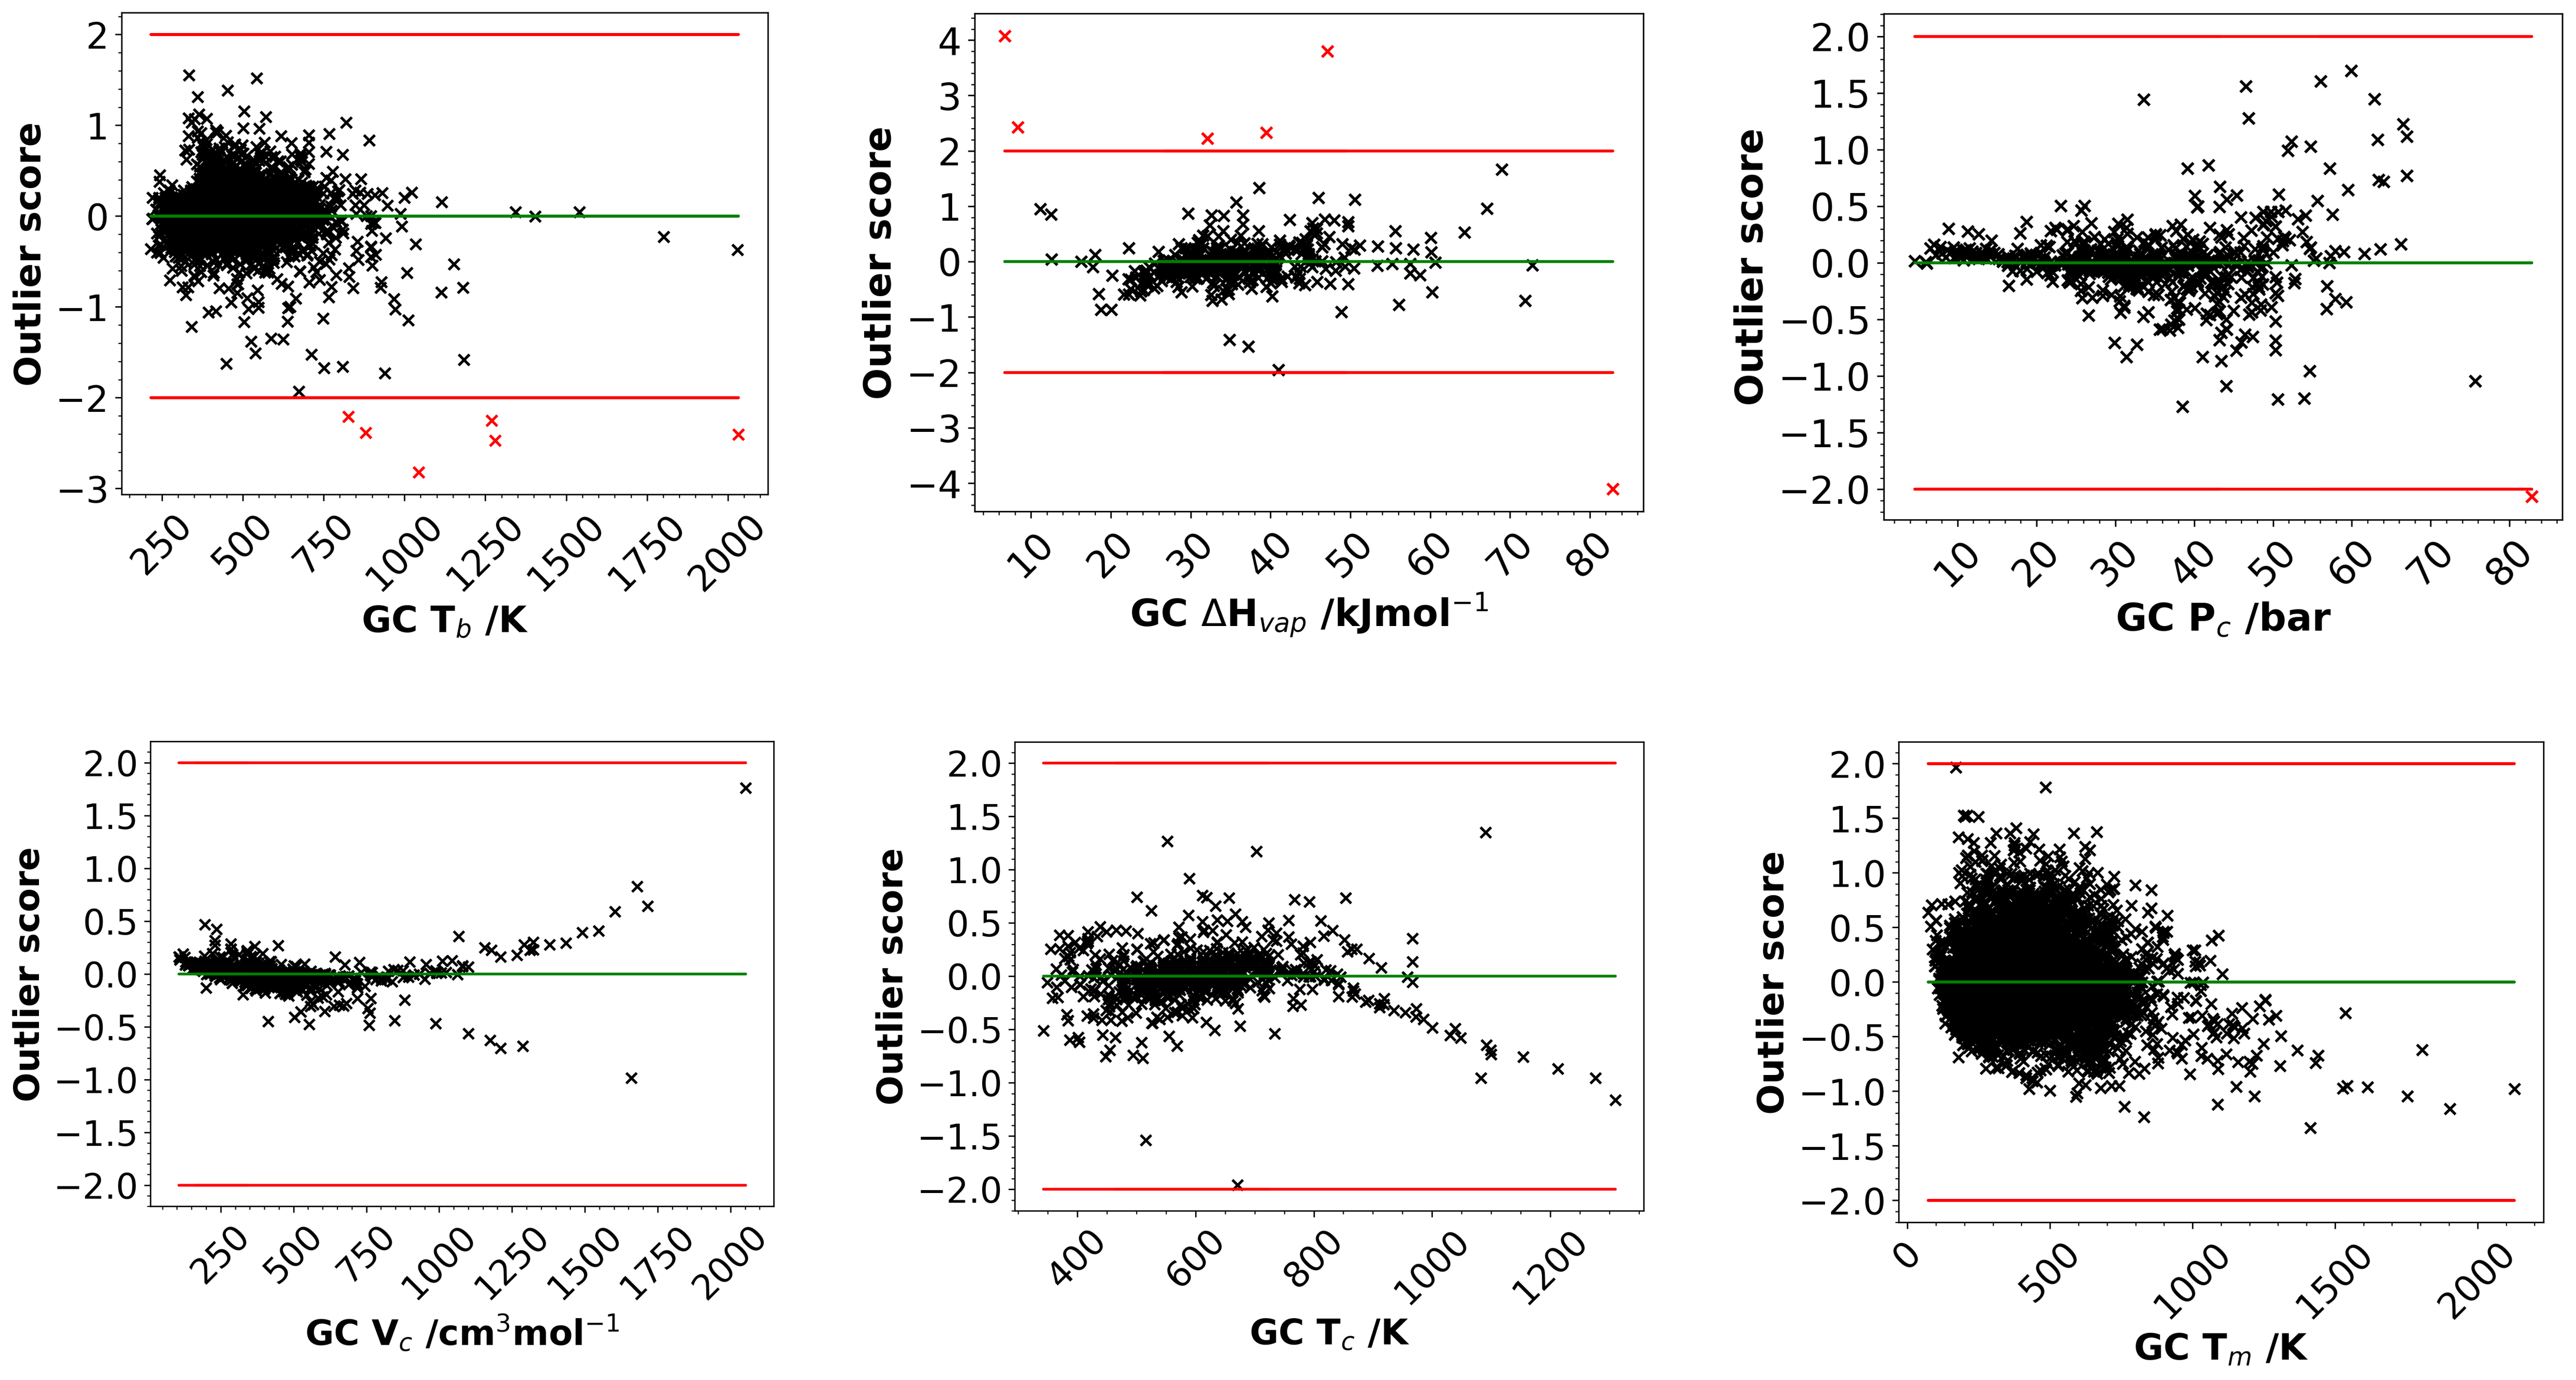
\includegraphics[width=1\linewidth]{images/outlier_score.png}
    \caption{Outlier scores. Scores scaled by one experimental data standard deviation.}
    \label{fig:outlier_scores}
\end{figure}




\begin{figure}[H]
    \centering
    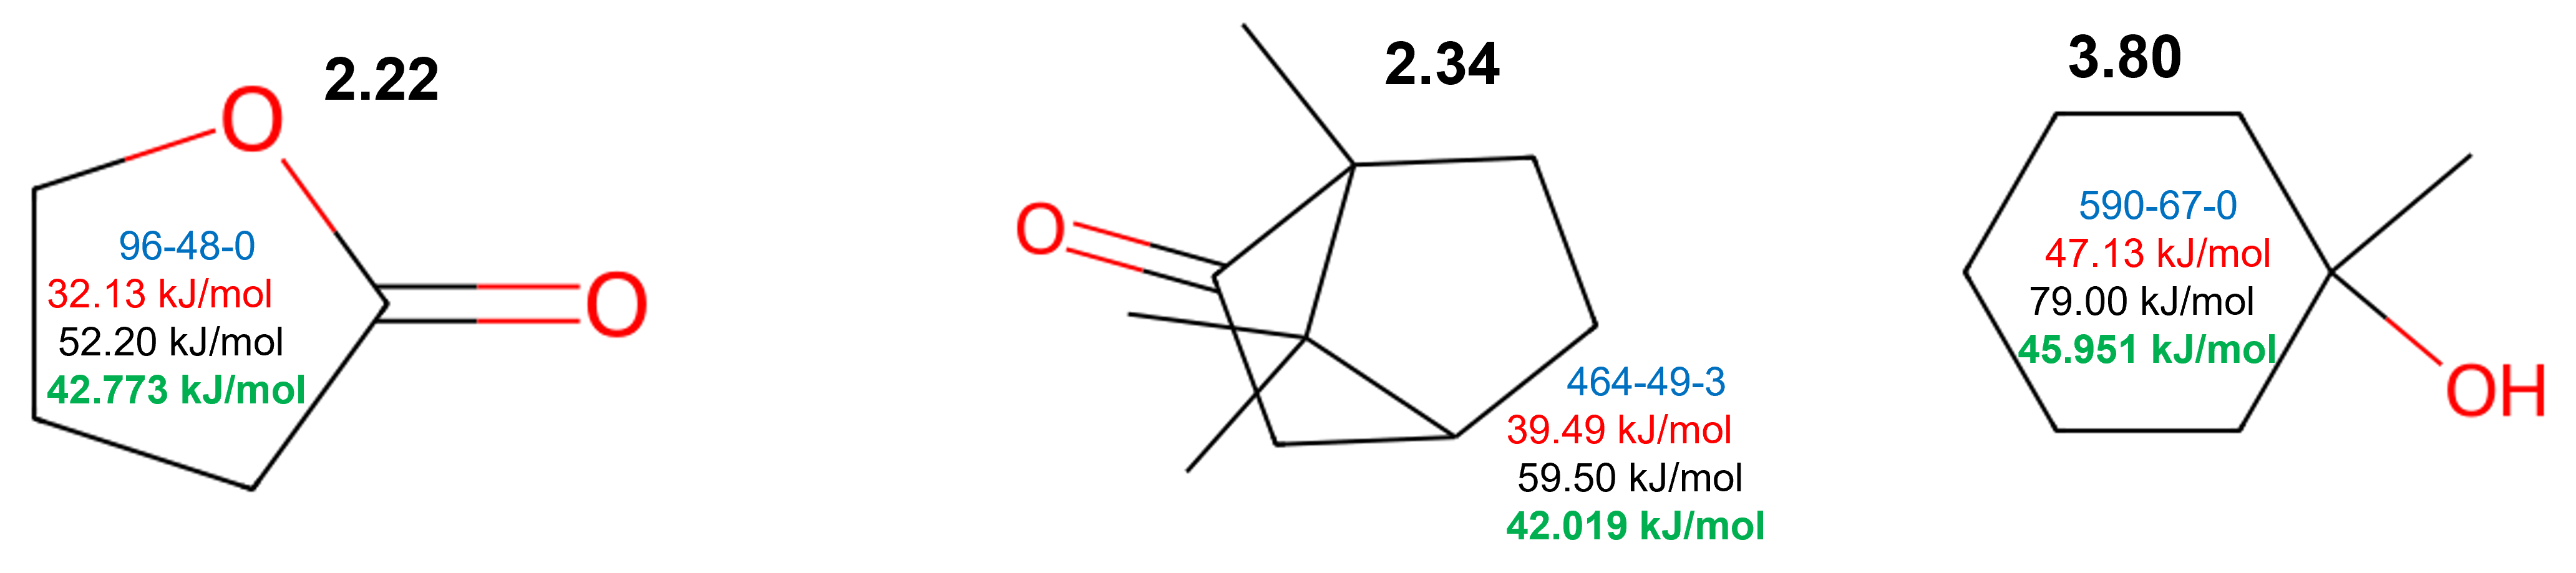
\includegraphics[width=1\linewidth]{images/bad_data_Hvap_molecules.png}
    \caption{Molecules with erroneous $\Delta$$H_{vap}$ data from CRC Handbook of Chemistry and Physics. Blue text is CAS number, red is JR GC predictions, black is CRC Handbook data and green is Yaws' critical properties handbook data.}
    \label{fig:molecules_with_erroneous_data}
\end{figure}


\begin{figure}[H]
    \centering
    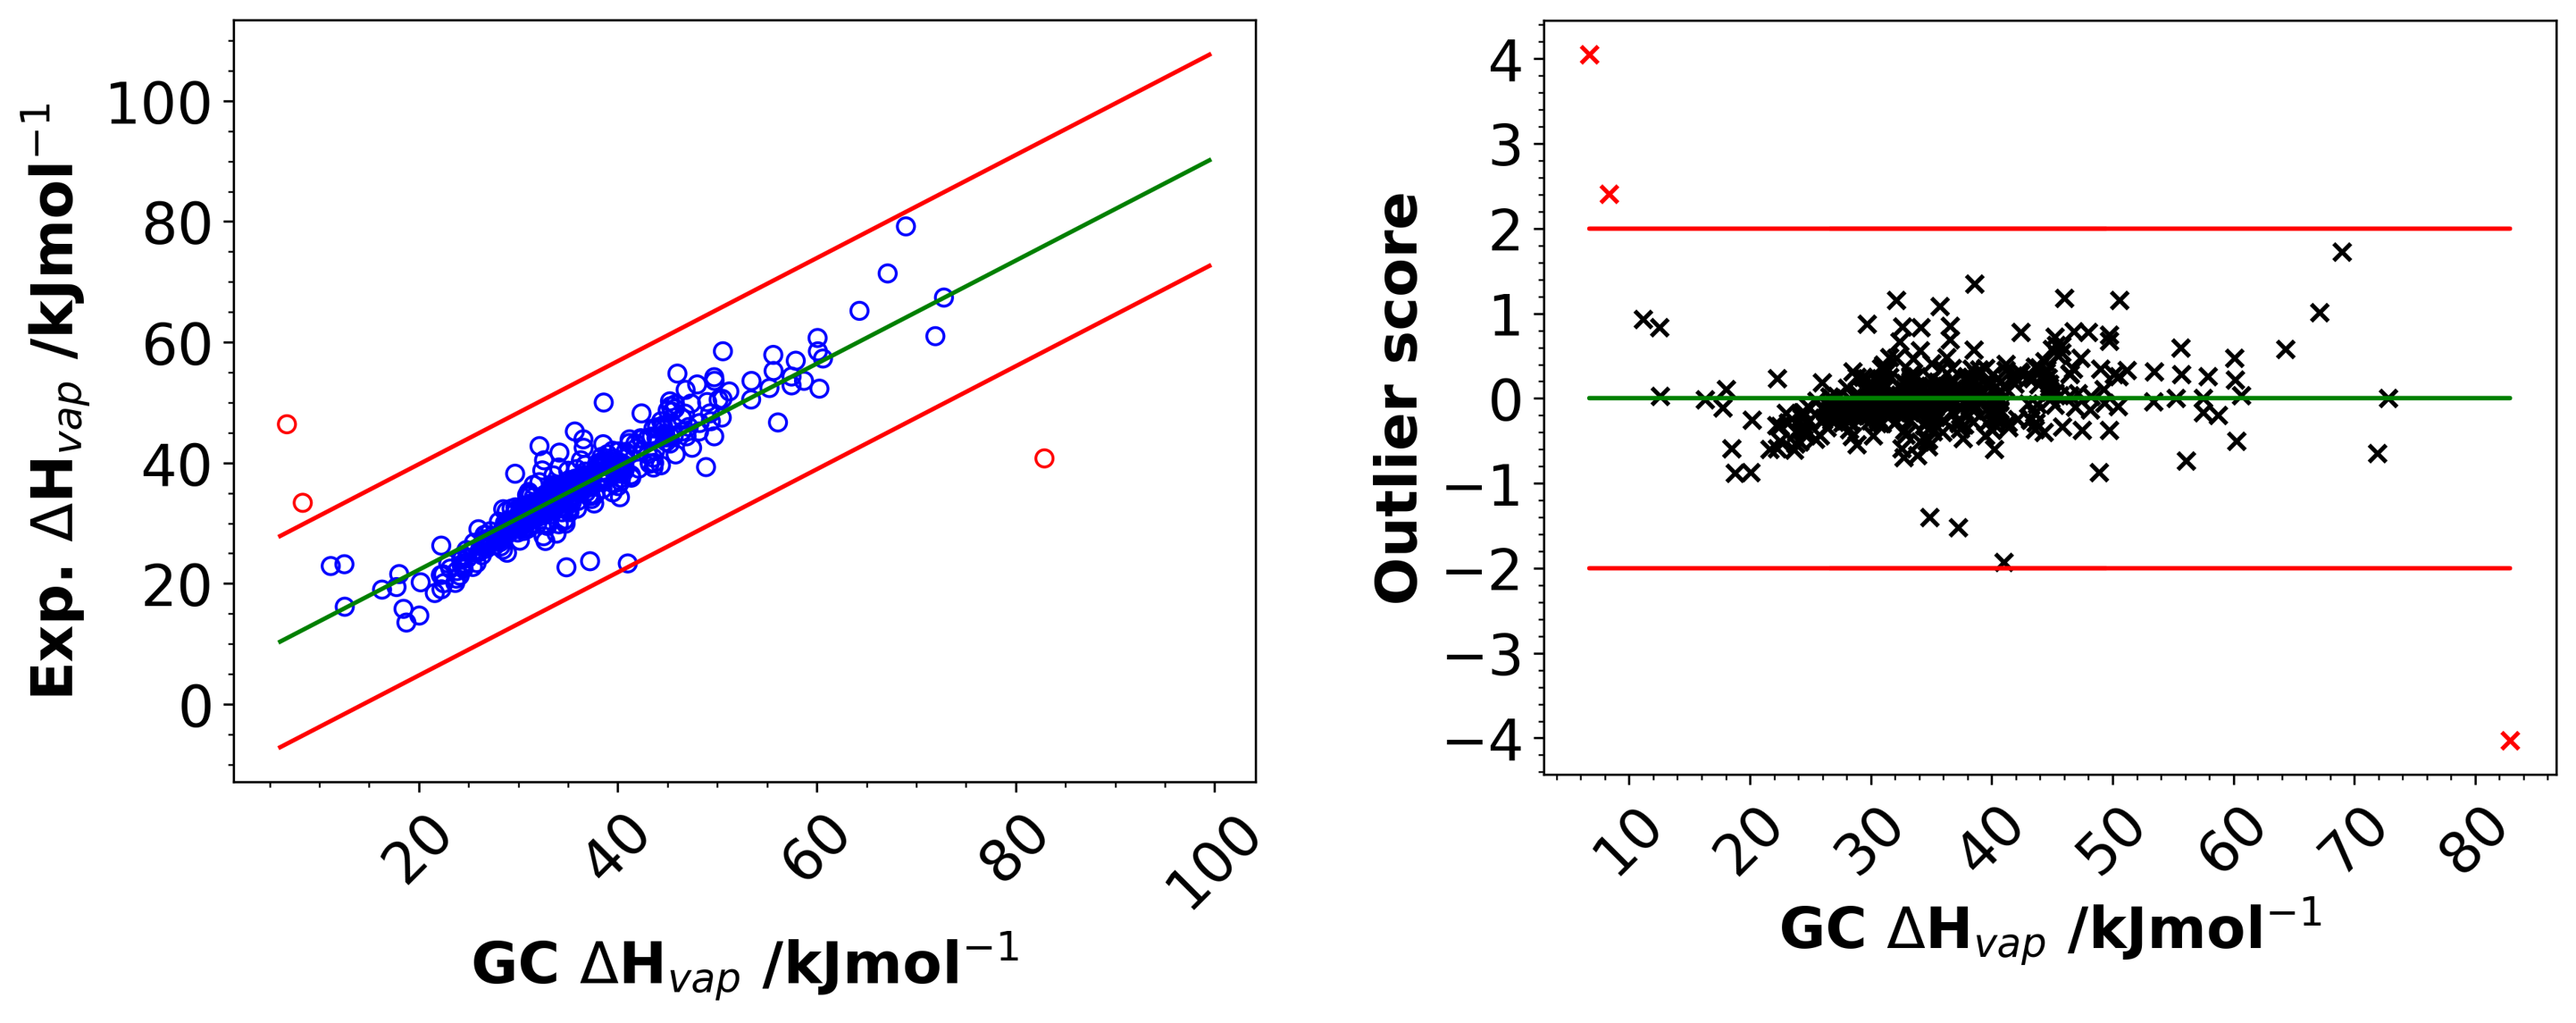
\includegraphics[width=0.5\linewidth]{images/Hvap_outlier_analysis_scores.png}
    \caption{$\Delta$$H_{vap}$  outlier analysis and scores after removing erroneous data from the CRC Handbook of Chemistry and Physics}
    \label{fig:enter-label}
\end{figure}





%\subsubsection{Analysis of feature vs label data (Montana and Kyla) }
% All extra 2D-only plots Montana made except Y_gc vs Y_exp plots go here with a brief discussion. (Y_gc vs Y_exp plots here will be duplicating 2D color-coded results in subsection 1 of results) 


\subsection{GP Model Screening}
%Talk about 5 model forms
We implemented five separate GP model structures to improve the results of JR GC predictions. Four of the models require both the GC property predictions $\mathbf{y_{GC}}$ and molecular weights ($\mathbf{M.W}$) and one only requires ($\mathbf{M.W}$) as an input. Each model makes different assumptions about the relationship between the input features and experimental property data $\mathbf{y_{\text{exp}}}$. We denote $\mathbf{X} = [\mathbf{y_{GC}}, \mathbf{M.W}]$

Model 1 described by equation \eqref{eq: Method_1} represents the most na\"ive approach to GP modeling in which we attempt to model $\mathbf{y_{\text{exp}}}$ using $m=0$. This method is best suited for models where trends in the data are unknown or difficult to elucidate and rely on the kernel function to do fully describe trends in the data.

\begin{equation}
    \mathbf{y_{\text{exp}}} \sim  GP = \mathcal{N}\left(\mathbf{y_{GC}}, K(\mathbf{X}) \right)
    \label{eq: Method_1}
\end{equation}

Model 2 and Model 3, represented by equations \eqref{Method_2} and \eqref{Method_3} respectively, attempt to model the discrepancy between the GC predictions and experimental data using a GP and are classified as traditional hybrid models. This method form is well-suited for properties where there is a clear correlation between the bias of the GC predictions and the experimental data. For a more robust implementation of this method, a mean function describing the bias with respect to input parameters should be added when clear. This model uses $m=0$, which reflects our belief that for GC models which are fairly accurate, bias should be negligible. The difference between \eqref{Method_2} and \eqref{Method_3} is that \eqref{Method_2} models discrepancy as a function of only $\mathbf{M.W}$.

\begin{equation}
    \mathbf{y_{\text{exp}}} - \mathbf{y_{GC}} = GP \sim \mathcal{N}\left(0, K(\mathbf{M.W}) \right)
    \label{Method_2}
\end{equation}


\begin{equation}
    \mathbf{y_{\text{exp}}} - \mathbf{y_{GC}} = GP \sim \mathcal{N}\left(0, K(\mathbf{X}) \right)
    \label{Method_3}
\end{equation}

The fourth GP model implementation (Model 4) in \eqref{Method_4} is the final model implementation which assumes $m = \mathbf{y_{GC}}$. This method is most suitable for property prediction data where $\mathbf{y_{GC}}$ is at least a somewhat faithful representation of $\mathbf{y_{\text{exp}}}$ and the relationship between $M.W$ and $\mathbf{y_{\text{exp}}}$ is unknown. We note that because $\mathbf{y_{GC}}$ is not a stochastic function, Method 4 and Method 3 are mathematically equivalent. Therefore, Method 4 is a hybrid model and equivalent to method 3. These models also produce the same results within a small numerical tolerance. 

\begin{equation}
    \mathbf{y_{\text{exp}}} \sim  GP = \mathcal{N}\left(\mathbf{y_{GC}}, K(\mathbf{X}) \right)
    \label{Method_4}
\end{equation}

The fifth GP model form (Model 5) in \eqref{Method_5} is a generalization of \eqref{Method_4} which includes tunable hyperparameters $A$ and $b$ in the mean function such that $m(\mathbf{x} \vert \mathbf{A},\mathbf{b}) = \mathbf{A}\mathbf{x} + \mathbf{b}$. This model is well suited for property predictions where the correlation of $M.W$ and $\mathbf{y_{\text{exp}}}$ is linear or when $\mathbf{y_{GC}}$ is a poor estimator of $\mathbf{y_{\text{exp}}}$. We note that because 

\begin{equation}
    \mathbf{y_{\text{exp}}} \sim GP = \mathcal{N}\left( \beta_{0} \mathbf{M.W} + \beta_{1} \mathbf{y_{GC}} +\beta_{2} , K(\mathbf{X}) \right)
    \label{eq: Method_5}
\end{equation}


% The five methods (4 above and the final method) were implemented to predict heat of vaporization ($H_{vap}$  $\frac{kJ}{mol}$), melting temperature ($T_m$ (K)), boiling temperature ($T_b$ ($K$)), and critical volume ($V_c$ ($\frac{cm^3}{mol}$), temperature ($T_c$ ($K$)), and pressure ($P_c$ ($bar$)). For the initial implementation a SE kernel with an isotropic length scale and a white kernel was used. The set of hyperparameters with the lowest log likelihood was used to make predictions. From our analysis, we concluded that \eqref{Method_2} was not very useful as molecular weight alone was not informative enough to describe the discrepancy. This was indicated by high MAPD values. \eqref{Method_4} and \eqref{Method_5} often performed similarly with \eqref{Method_1} performing marginally worse. In the case where there was a strong correlation between discrepancy and the input features, \eqref{Method_3} yielded the lowest MAPD values. A table of the preliminary results can be found in the SI.

\subsection{Kernel Function Screening}

Section XX in the main text are the results of examining the effect of different kernels. Here, we elaborate on the different kernels. For this section, $d(\mathbf{x}, \mathbf{x}^{\prime})$ is the euclidean distance between data $\mathbf{x}$ and $\mathbf{x}^{\prime}$.

The squared exponential kernel, also known as the radial basis function (RBF) is described by \eqref{se}. It assumes the underlying function is infinitely differentiable and is most useful for smooth functions.

\begin{equation}
    k(\mathbf{x}, \mathbf{x}^{\prime}) = \exp\left(-\frac{d(\mathbf{x}, \mathbf{x}^{\prime})^2}{2\ell^2} \right)
    \label{se}
\end{equation}

The Mat\`ern kernels are defined by their smoothness, $\nu$, and length scale $\ell$. As $\nu \rightarrow \infty$ the Mat\`ern kernel becomes equivalent to the RBF kernel and is thus a generalization of the RBF kernel. The general form of the Mat\`ern kernel is provided in \eqref{Matern} where $K_\nu(\cdot)$ is the modified Bessel function and $\Gamma(\cdot)$ is the gamma function. This kernel is a particularly good choice for functions which are differentiable a certain number of times.

\begin{equation}
    k_\nu(\mathbf{x}, \mathbf{x}^{\prime}, \nu) = \frac{2^{1-\nu}}{\Gamma(\nu)} \left( \sqrt{2\nu} \frac{d(\mathbf{x}, \mathbf{x}^{\prime})}{\ell} \right)^\nu K_\nu \left( \sqrt{2\nu} \frac{d(\mathbf{x}, \mathbf{x}^{\prime})}{\ell} \right)
    \label{Matern}
\end{equation}

The rational quadratic kernel described by \eqref{rq_kernel} is a hybrid is infinitely mean-square differentiable \cite{Gramacy2020Surrogates:Sciences} and is a more general form of the RBF kernel. Because the parameter $\alpha$ can be tuned, this function is equipped to handle functions with varying levels of smoothness. This is the kernel function implemented in our final model.

\begin{equation}
    k(\mathbf{x}, \mathbf{x}^{\prime}) = \left(1 + \frac{d(\mathbf{x}, \mathbf{x}^{\prime})^2}{2\alpha l^2}\right)^{-\alpha}
    \label{rq_kernel}
\end{equation}


% The power exponential kernels are popular due to good numerical stability from better covariance matrix condition numbers. Particularly common is the Gaussian kernel, in which hyperparameter $\alpha$ is set to $\alpha = 2$ \cite{Gramacy2020Surrogates:Sciences}. 

% \begin{equation}
%     k_{\alpha}(\mathbf{x}, \mathbf{x}^{\prime}, \nu) = \exp \Biggl\{- \left( \frac{d(\mathbf{x}, \mathbf{x}^{\prime})}{\sqrt{\ell}} \right)^\alpha \Biggl\} \text{for $0<\alpha \leq 2$,}
%     \label{Exp_kernel}
% \end{equation}


Note, hyperparameters $\alpha$ and $\ell$ in these equations must be optimized based on the training data. We also note that any kernel listed can be either isotropic or anisotropic meaning that length scale $\ell$ is either a scalar or a vector with the same number of dimensions as $\mathbf{x}$.



\section{Results and Discussion}

\subsection{GC-GP hybrid models accurately predict properties and correct systematic bias}

% plots with error bars
\begin{figure}[H]
    \centering
    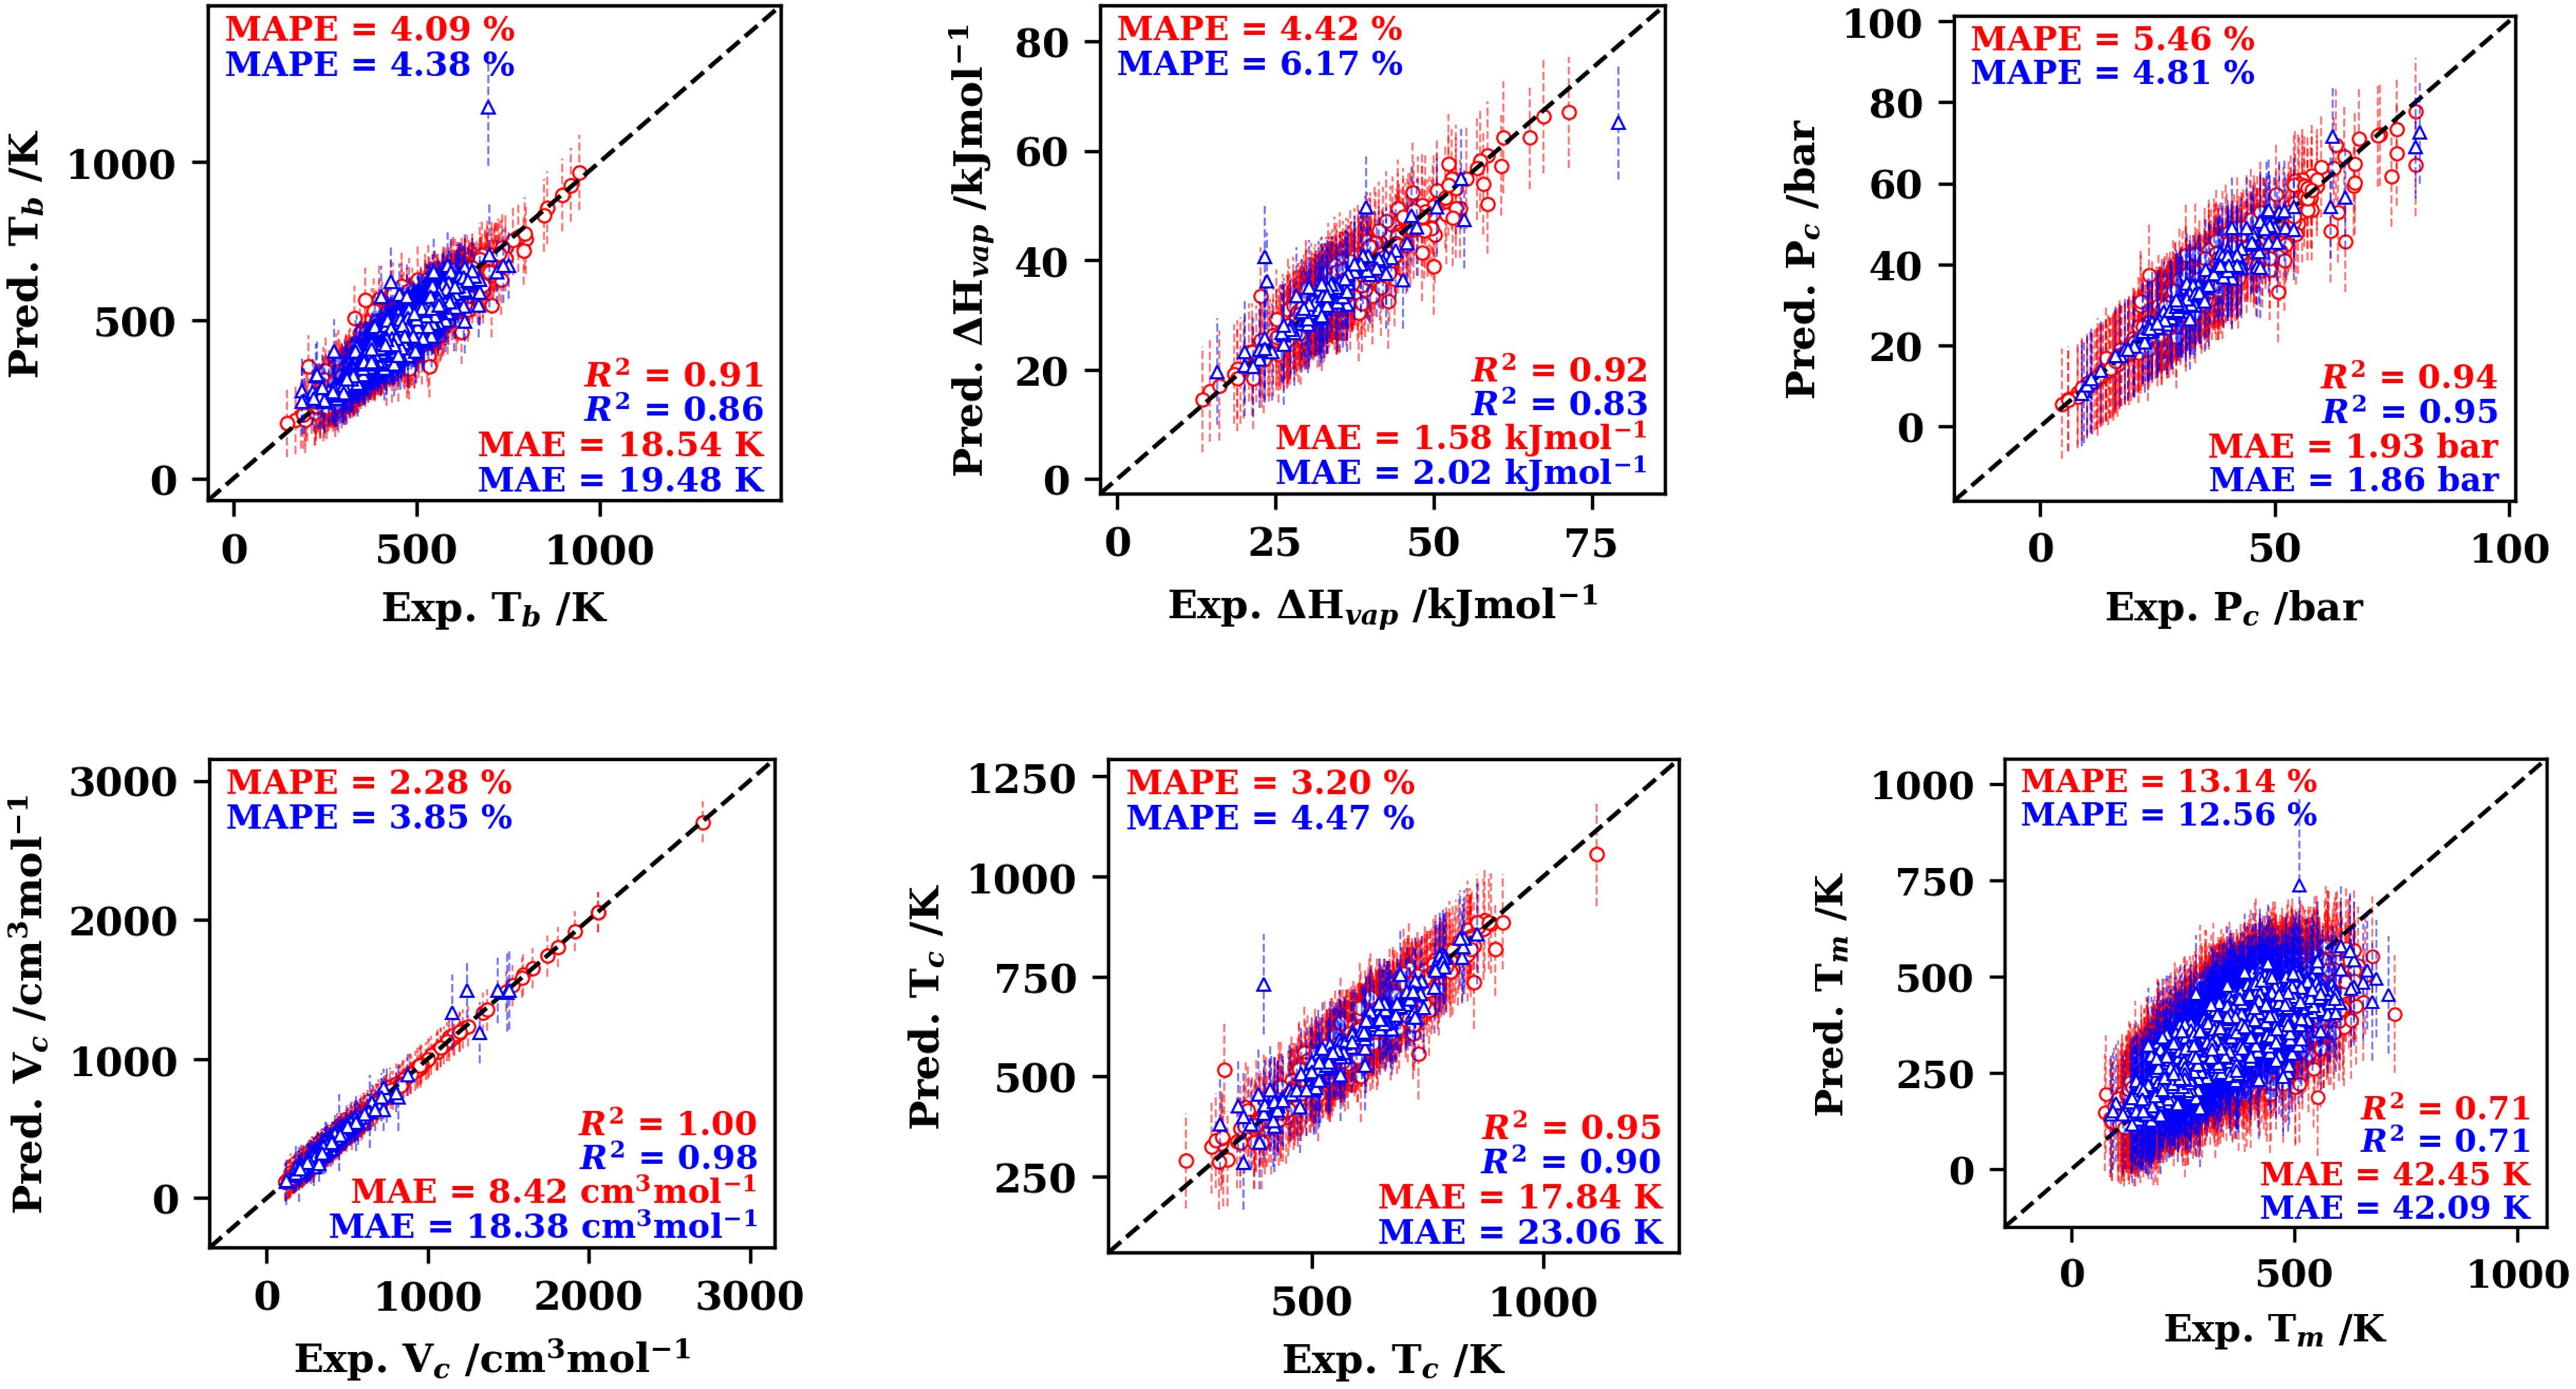
\includegraphics[width=1\linewidth]{images/2D_GCGP_pred_results_SI.png}
    \caption{GCGP method results with 95 \% confidence error bars}
    \label{fig:GCGP_with_error_bars}
\end{figure}





\begin{table}[H]
    \centering
    \begin{tabular}{cccccc}
         Property&  length scale&  shape parameter&  RQ kernel variance&  White kernel variance&  LML
\\
         $T_b$&  2.940&  0.006&  29.878&  0.098&  -1207.450
\\
         $H_{vap}$&  3.041&  0.215&  8.881&  0.082&  -121.687
\\
         $P_c$&  1.944&  4997.324&  0.827&  0.065&  -54.133
\\
         $V_c$&  0.514&  0.072&  0.324&  0.002&  662.185
\\
         $T_c$&  2.061&  0.348&  1.638&  0.052&  -15.877
\\
         $T_m$&  5.557&  0.021&  20.158&  0.294&  -4094.385
\\
    \end{tabular}
    \caption{Caption}
    \label{tab:my_label}
\end{table}





\begin{table}[H]
    \centering
    \begin{tabular}{ccccccc}
         &  Train&  &  &  Test&  & 
\\
         variance hyperparameter setting&  R2 &  MAPD&  MAE&  R2 &  MAPD& MAE
\\
         Start at 1e-5 and optimize&  0.71&  12.95&  42.08&  0.7&  13.3& 43.21
\\
         Fix at value corresponding to 1 K &  0.98&  1.82&  6.02&  0.7&  13.06& 42.59
\\
         Fix at value corresponding to 10 K &  0.98&  1.89&  6.25&  0.7&  13.05& 42.56
\\
         This work&  0.71&  13.14&  42.45&  0.71&  12.56& 42.09
\\
    \end{tabular}
    \caption{Caption}
    \label{tab:my_label}
\end{table}
% Discussion and table showing effect of white noise kernel settings on Tm model training 


\subsection{GC-GP hybrid model performance is robust across kernel and structure choices (Barnabas) }
% Six big tables showing model performance metrics across all model-kernel (50 in total) combinations for all properties - one per property
%$\Delta H_{vap}$

\begin{table}[H]
    \centering
    \begin{tabular}{>{\raggedright\arraybackslash}p{0.1cm}>{\raggedright\arraybackslash}p{3.7cm}>{\centering\arraybackslash}p{0.90cm}>{\centering\arraybackslash}p{0.90cm}>{\centering\arraybackslash}p{0.90cm}>{\centering\arraybackslash}p{0.90cm}>{\centering\arraybackslash}p{0.90cm}>{\centering\arraybackslash}p{0.90cm}>{\centering\arraybackslash}p{0.90cm}>{\centering\arraybackslash}p{0.90cm}>{\centering\arraybackslash}p{0.90cm}>{\centering\arraybackslash}p{0.90cm}}
  &&\multicolumn{10}{c}{\textbf{$\Delta H_{vap}$}}\\
  && Mt12& Mt12    (2)& Mt32& Mt32    (2)& Mt52& Mt52     (2)& RBF& RBF 
   (2)& RQ&RQ    (2)
\\
  1&Tst MAPD /\%& 6.175& 6.014& 6.267& 5.894& 6.206& 5.845& 6.401& 5.819& 6.136&5.816
\\
  &Trn MAPD /\%& 3.335& 3.665& 4.407& 4.521& 4.480& 4.606& 4.727& 4.677& 4.446&4.662
\\
  &Tst MAE /$kJmol^{-1}$& 2.006& 1.941& 2.048& 1.916& 2.033& 1.905& 2.097& 1.898& 2.015&1.897
\\
  &Trn MAE /$kJmol^{-1}$& 1.196& 1.299& 1.577& 1.598& 1.599& 1.625& 1.692& 1.644& 1.585&1.639
\\
  &Tst R2& 0.823& 0.844& 0.828& 0.848& 0.830& 0.847& 0.821& 0.847& 0.832&0.847
\\
  &Trn R2& 0.956& 0.950& 0.925& 0.923& 0.923& 0.920& 0.914& 0.918& 0.924&0.919
\\
  &LML& -131& -116& -119& -105& -118& -103& -122& -103& -119&-103
\\
  2&Tst MAPD /\%& 6.881& 6.881& 7.072& 6.322& 7.105& 6.331& 7.245& 6.337& 6.337&6.337
\\
  &Trn MAPD /\%& 3.799& 3.799& 4.122& 5.337& 4.172& 5.389& 4.178& 5.386& 5.386&5.386
\\
  &Tst MAE /$kJmol^{-1}$& 2.235& 2.235& 2.287& 2.067& 2.294& 2.070& 2.333& 2.072& 2.072&2.072
\\
  &Trn MAE /$kJmol^{-1}$& 1.362& 1.362& 1.473& 1.897& 1.490& 1.914& 1.490& 1.914& 1.914&1.914
\\
  &Tst R2& 0.793& 0.793& 0.785& 0.839& 0.785& 0.838& 0.778& 0.837& 0.837&0.837
\\
  &Trn R2& 0.941& 0.941& 0.933& 0.836& 0.931& 0.834& 0.931& 0.834& 0.834&0.834
\\
  &LML& -477& -477& -475& -492& -474& -492& -473& -491& -491&-491
\\
  3&Tst MAPD /\%& 6.190& 6.015& 6.290& 5.877& 6.249& 5.822& 6.376& 5.796& 6.166&5.797
\\
  &Trn MAPD /\%& 3.258& 3.471& 4.417& 4.516& 4.500& 4.605& 4.754& 4.634& 4.425&4.632
\\
  &Tst MAE /$kJmol^{-1}$& 2.006& 1.936& 2.054& 1.907& 2.045& 1.895& 2.087& 1.882& 2.024&1.885
\\
  &Trn MAE /$kJmol^{-1}$& 1.171& 1.231& 1.584& 1.597& 1.611& 1.624& 1.707& 1.632& 1.583&1.632
\\
          &Tst R2&  0.824&  0.846&  0.827&  0.849&  0.828&  0.848&  0.821&   0.851&0.830& 0.850
\\
          &Trn R2&  0.957&  0.955&  0.925&  0.923&  0.922&  0.920&  0.912&   0.919&0.924& 0.919
\\
          &LML&  -405&  -394&  -393&  -378&  -394&  -377&  -397&   -376&-393& -376
\\
          4&Tst MAPD /\%&  6.190&  6.012&  6.290&  5.871&  6.244&  5.824&  6.387&   5.797&6.168& 5.797
\\
          &Trn MAPD /\%&  3.296&  3.499&  4.414&  4.521&  4.488&  4.603&  4.743&   4.635&4.424& 4.633
\\
          &Tst MAE /$kJmol^{-1}$&  2.007&  1.936&  2.054&  1.906&  2.044&  1.895&  2.091&   1.882&2.025& 1.885
\\
          &Trn MAE /$kJmol^{-1}$&  1.184&  1.241&  1.583&  1.598&  1.606&  1.624&  1.703&   1.633&1.582& 1.632
\\
          &Tst R2&  0.824&  0.846&  0.827&  0.849&  0.828&  0.848&  0.821&   0.851&0.830& 0.850
\\
          &Trn R2&  0.956&  0.954&  0.925&  0.922&  0.922&  0.920&  0.913&   0.919&0.924& 0.919
\\
  &LML& -133& -122& -122& -107& -122& -106& -126& -105& -122&-105
\\
  5&Tst MAPD /\%& 6.182& 5.932& 6.290& 5.857& 6.236& 5.823& 6.056& 5.776& 6.089&5.776
\\
  &Trn MAPD /\%& 3.475& 3.794& 4.350& 4.518& 4.399& 4.601& 4.397& 4.652& 4.400&4.652
\\
  &Tst MAE /$kJmol^{-1}$& 2.009& 1.908& 2.054& 1.900& 2.042& 1.894& 1.999& 1.878& 2.007&1.878
\\
  &Trn MAE /$kJmol^{-1}$& 1.248& 1.345& 1.558& 1.596& 1.573& 1.621& 1.569& 1.635& 1.570&1.635
\\
  &Tst R2& 0.824& 0.852& 0.827& 0.851& 0.829& 0.850& 0.832& 0.851& 0.832&0.851
\\
  &Trn R2& 0.952& 0.946& 0.927& 0.922& 0.925& 0.920& 0.925& 0.919& 0.925&0.919
\\
  &LML& -125& -111& -116& -102& -115& -101& -114& -99& -114&-99
\\
  && & & & & & & & & &\\
    \end{tabular}
    \caption{Caption}
    \label{tab:my_label}
\end{table}




%%%%%%%%%%%%%%%%%% Pc
\begin{table}[H]
    \centering
    \begin{tabular}{>{\raggedright\arraybackslash}p{0.1cm}>{\raggedright\arraybackslash}p{3.7cm}>{\centering\arraybackslash}p{0.90cm}>{\centering\arraybackslash}p{0.90cm}>{\centering\arraybackslash}p{0.90cm}>{\centering\arraybackslash}p{0.90cm}>{\centering\arraybackslash}p{0.90cm}>{\centering\arraybackslash}p{0.90cm}>{\centering\arraybackslash}p{0.90cm}>{\centering\arraybackslash}p{0.90cm}>{\centering\arraybackslash}p{0.90cm}>{\centering\arraybackslash}p{0.90cm}}
  &&\multicolumn{10}{c}{\textbf{$P_{c}$}}\\
  && Mt12& Mt12    (2)& Mt32& Mt32    (2)& Mt52& Mt52     (2)& RBF& RBF 
   (2)& RQ&RQ    (2)
\\
  1&Tst MAPD /\%& 5.257& 5.268& 4.801& 4.836& 4.761& 4.816& 4.797& 4.853& 4.788&4.830
\\
  &Trn MAPD /\%& 4.632& 4.708& 5.476& 5.453& 5.514& 5.523& 5.540& 5.518& 5.526&5.516
\\
  &Tst MAE /bars& 2.026& 2.031& 1.871& 1.884& 1.858& 1.881& 1.870& 1.898& 1.862&1.889
\\
  &Trn MAE /bars& 1.603& 1.635& 1.922& 1.922& 1.941& 1.952& 1.947& 1.956& 1.943&1.955
\\
  &Tst R2& 0.941& 0.940& 0.945& 0.944& 0.945& 0.944& 0.945& 0.944& 0.945&0.944
\\
  &Trn R2& 0.957& 0.955& 0.938& 0.938& 0.937& 0.937& 0.937& 0.937& 0.937&0.937
\\
  &LML& -78& -78& -61& -61& -60& -59& -61& -59& -60&-59
\\
  2&Tst MAPD /\%& 6.337& 6.337& 6.381& 6.381& 6.385& 6.385& 6.388& 6.388& 6.388&6.388
\\
  &Trn MAPD /\%& 6.484& 6.484& 6.725& 6.725& 6.725& 6.725& 6.717& 6.717& 6.717&6.717
\\
  &Tst MAE /bars& 2.325& 2.325& 2.354& 2.354& 2.354& 2.354& 2.352& 2.352& 2.352&2.352
\\
  &Trn MAE /bars& 2.200& 2.200& 2.278& 2.278& 2.279& 2.279& 2.278& 2.278& 2.278&2.278
\\
  &Tst R2& 0.918& 0.918& 0.917& 0.917& 0.917& 0.917& 0.918& 0.918& 0.918&0.918
\\
  &Trn R2& 0.920& 0.920& 0.915& 0.915& 0.915& 0.915& 0.915& 0.915& 0.915&0.915
\\
  &LML& -766& -766& -766& -766& -766& -766& -766& -766& -766&-766
\\
  3&Tst MAPD /\%& 5.177& 5.099& 4.827& 4.832& 4.781& 4.780& 4.800& 4.806& 4.800&4.806
\\
  &Trn MAPD /\%& 4.862& 4.840& 5.405& 5.415& 5.443& 5.449& 5.465& 5.469& 5.465&5.469
\\
  &Tst MAE /bars& 1.989& 1.967& 1.873& 1.874& 1.857& 1.854& 1.858& 1.857& 1.858&1.857
\\
  &Trn MAE /bars& 1.713& 1.701& 1.910& 1.912& 1.927& 1.926& 1.935& 1.935& 1.935&1.935
\\
          &Tst R2&  0.942&  0.944&  0.945&  0.945&  0.945&  0.945&  0.945&   0.945&0.945& 0.945
\\
          &Trn R2&  0.950&  0.951&  0.938&  0.938&  0.937&  0.937&  0.937&   0.937&0.937& 0.937
\\
          &LML&  -717&  -716&  -709&  -709&  -707&  -707&  -705&   -705&-705& -705
\\
          4&Tst MAPD /\%&  5.191&  5.116&  4.824&  4.828&  4.783&  4.779&  4.806&   4.807&4.806& 4.807
\\
          &Trn MAPD /\%&  4.838&  4.805&  5.401&  5.409&  5.438&  5.442&  5.458&   5.459&5.458& 5.459
\\
          &Tst MAE /bars&  1.992&  1.970&  1.872&  1.873&  1.858&  1.854&  1.860&   1.860&1.860& 1.860
\\
          &Trn MAE /bars&  1.706&  1.691&  1.910&  1.911&  1.927&  1.926&  1.935&   1.935&1.935& 1.935
\\
          &Tst R2&  0.942&  0.944&  0.945&  0.945&  0.945&  0.945&  0.945&   0.945&0.945& 0.945
\\
          &Trn R2&  0.950&  0.952&  0.938&  0.938&  0.937&  0.937&  0.937&   0.937&0.937& 0.937
\\
  &LML& -67& -65& -57& -57& -55& -55& -54& -54& -54&-54
\\
  5&Tst MAPD /\%& 5.126& 5.085& 4.848& 4.848& 4.779& 4.789& 4.795& 4.793& 4.795&4.793
\\
  &Trn MAPD /\%& 5.009& 4.993& 5.448& 5.448& 5.479& 5.484& 5.508& 5.511& 5.508&5.511
\\
  &Tst MAE /bars& 1.979& 1.965& 1.882& 1.882& 1.857& 1.859& 1.854& 1.851& 1.854&1.851
\\
  &Trn MAE /bars& 1.744& 1.735& 1.913& 1.913& 1.929& 1.929& 1.939& 1.938& 1.939&1.938
\\
  &Tst R2& 0.942& 0.944& 0.945& 0.945& 0.945& 0.945& 0.946& 0.946& 0.946&0.946
\\
  &Trn R2& 0.949& 0.950& 0.938& 0.938& 0.937& 0.938& 0.937& 0.937& 0.937&0.937
\\
  &LML& -62& -61& -56& -56& -54& -54& -53& -53& -53&-53
\\
  && & & & & & & & & &\\
    \end{tabular}
    \caption{Caption}
    \label{tab:my_label}
\end{table}

%>>>>> Vc
\begin{table}[H]
    \centering
    \begin{tabular}{>{\raggedright\arraybackslash}p{0.1cm}>{\raggedright\arraybackslash}p{4.0cm}>{\centering\arraybackslash}p{0.90cm}>{\centering\arraybackslash}p{0.90cm}>{\centering\arraybackslash}p{0.90cm}>{\centering\arraybackslash}p{0.90cm}>{\centering\arraybackslash}p{0.90cm}>{\centering\arraybackslash}p{0.90cm}>{\centering\arraybackslash}p{0.90cm}>{\centering\arraybackslash}p{0.90cm}>{\centering\arraybackslash}p{0.90cm}>{\centering\arraybackslash}p{0.90cm}}
  &&\multicolumn{10}{c}{\textbf{$V_{c}$}}\\
  && Mt12& Mt12    (2)& Mt32& Mt32    (2)& Mt52& Mt52     (2)& RBF& RBF 
   (2)& RQ&RQ    (2)
\\
  1&Tst MAPD /\%& 3.735& 3.730& 4.162& 4.133& 3.693& 3.701& 3.560& 3.588& 3.675&3.704
\\
  &Trn MAPD /\%& 1.220& 1.239& 2.427& 2.401& 3.129& 3.127& 3.211& 3.218& 3.161&3.158
\\
  &Tst MAE /$cm^{3}mol^{-1}$& 17.385& 17.464& 20.988& 20.691& 17.672& 17.720& 17.045& 17.148& 17.620&17.832
\\
  &Trn MAE /$cm^{3}mol^{-1}$& 4.739& 4.797& 9.034& 8.926& 12.486& 12.482& 12.911& 12.983& 12.639&12.624
\\
  &Tst R2& 0.982& 0.981& 0.972& 0.973& 0.981& 0.981& 0.984& 0.984& 0.982&0.981
\\
  &Trn R2& 0.999& 0.999& 0.998& 0.998& 0.996& 0.996& 0.995& 0.995& 0.996&0.996
\\
  &LML& 613& 615& 631& 632& 606& 606& 599& 600& 606&606
\\
  2&Tst MAPD /\%& 4.425& 4.425& 4.341& 4.341& 4.314& 4.314& 4.276& 4.276& 4.514&4.514
\\
  &Trn MAPD /\%& 2.109& 2.109& 2.743& 2.743& 2.874& 2.874& 2.937& 2.937& 2.263&2.263
\\
  &Tst MAE /$cm^{3}mol^{-1}$& 20.341& 20.341& 20.239& 20.239& 20.218& 20.218& 20.224& 20.224& 20.366&20.366
\\
  &Trn MAE /$cm^{3}mol^{-1}$& 8.464& 8.464& 10.739& 10.739& 11.240& 11.240& 11.384& 11.384& 9.009&9.009
\\
  &Tst R2& 0.977& 0.977& 0.976& 0.976& 0.978& 0.978& 0.981& 0.981& 0.980&0.980
\\
  &Trn R2& 0.998& 0.998& 0.997& 0.997& 0.997& 0.997& 0.997& 0.997& 0.998&0.998
\\
  &LML& -455& -455& -475& -475& -480& -480& -484& -484& -471&-471
\\
  3&Tst MAPD /\%& 3.629& 3.594& 4.054& 3.948& 4.206& 4.088& 3.635& 4.206& 3.899&3.838
\\
  &Trn MAPD /\%& 1.425& 1.414& 2.297& 2.252& 2.429& 2.382& 3.151& 2.598& 2.311&2.283
\\
  &Tst MAE /$cm^{3}mol^{-1}$& 17.000& 16.714& 20.169& 19.357& 21.434& 20.527& 17.534& 21.877& 18.845&18.294
\\
  &Trn MAE /$cm^{3}mol^{-1}$& 5.526& 5.511& 8.509& 8.344& 8.923& 8.741& 12.599& 9.488& 8.509&8.409
\\
          &Tst R2&  0.982&  0.983&  0.974&  0.977&  0.970&  0.974&  0.982&   0.968&0.977& 0.979
\\
          &Trn R2&  0.999&  0.999&  0.998&  0.998&  0.998&  0.998&  0.996&   0.998&0.998& 0.998
\\
          &LML&  -312&  -311&  -315&  -313&  -325&  -323&  -351&   -349&-311& -309
\\
          4&Tst MAPD /\%&  3.629&  3.580&  3.947&  3.786&  4.044&  3.903&  3.608&   3.831&3.853& 3.760
\\
          &Trn MAPD /\%&  1.436&  1.425&  2.220&  2.166&  2.337&  2.291&  3.142&   2.303&2.281& 2.239
\\
          &Tst MAE /$cm^{3}mol^{-1}$&  16.965&  16.580&  19.137&  17.972&  19.746&  18.695&  17.364&   17.877&18.384& 17.612
\\
          &Trn MAE /$cm^{3}mol^{-1}$&  5.572&  5.562&  8.227&  8.052&  8.603&  8.437&  12.576&   8.401&8.421& 8.279
\\
          &Tst R2&  0.982&  0.983&  0.976&  0.980&  0.974&  0.978&  0.982&   0.980&0.978& 0.981
\\
          &Trn R2&  0.999&  0.999&  0.998&  0.999&  0.998&  0.998&  0.996&   0.998&0.998& 0.998
\\
  &LML& 658& 660& 662& 665& 658& 660& 620& 650& 662&665
\\
  5&Tst MAPD /\%& 3.622& 3.570& 3.884& 3.723& 3.964& 3.820& 3.576& 3.636& 3.826&3.725
\\
  &Trn MAPD /\%& 1.439& 1.428& 2.199& 2.143& 2.320& 2.272& 3.134& 3.137& 2.276&2.231
\\
  &Tst MAE /$cm^{3}mol^{-1}$& 16.884& 16.478& 18.582& 17.396& 19.027& 17.925& 17.201& 17.620& 18.136&17.296
\\
  &Trn MAE /$cm^{3}mol^{-1}$& 5.585& 5.575& 8.159& 7.976& 8.542& 8.365& 12.555& 12.578& 8.410&8.257
\\
  &Tst R2& 0.982& 0.983& 0.976& 0.980& 0.975& 0.978& 0.982& 0.982& 0.979&0.981
\\
  &Trn R2& 0.999& 0.999& 0.999& 0.999& 0.998& 0.998& 0.996& 0.996& 0.998&0.998
\\
  &LML& 661& 663& 666& 669& 662& 665& 621& 623& 665&668
\\
  && & & & & & & & & &\\
    \end{tabular}
    \caption{Caption}
    \label{tab:my_label}
\end{table}



%%%%%%%%%%%%%%%%%%%% Tc
\begin{table}[H]
    \centering
    \begin{tabular}{>{\raggedright\arraybackslash}p{0.1cm}>{\raggedright\arraybackslash}p{3.0cm}>{\centering\arraybackslash}p{0.90cm}>{\centering\arraybackslash}p{0.90cm}>{\centering\arraybackslash}p{0.90cm}>{\centering\arraybackslash}p{0.90cm}>{\centering\arraybackslash}p{0.90cm}>{\centering\arraybackslash}p{0.90cm}>{\centering\arraybackslash}p{0.90cm}>{\centering\arraybackslash}p{0.90cm}>{\centering\arraybackslash}p{0.90cm}>{\centering\arraybackslash}p{0.90cm}}
  &&\multicolumn{10}{c}{\textbf{$T_{c}$}}\\
  && Mt12& Mt12    (2)& Mt32& Mt32    (2)& Mt52& Mt52     (2)& RBF& RBF 
   (2)& RQ&RQ    (2)
\\
  1&Tst MAPD /\%& 4.240& 4.239& 4.468& 4.455& 4.492& 4.475& 4.577& 4.575& 4.489&4.476
\\
  &Trn MAPD /\%& 2.369& 2.442& 3.208& 3.208& 3.242& 3.256& 3.532& 3.541& 3.219&3.231
\\
  &Tst MAE /K& 21.889& 22.004& 23.121& 23.091& 23.212& 23.171& 23.866& 23.805& 23.141&23.123
\\
  &Trn MAE /K& 13.277& 13.705& 17.942& 17.948& 18.093& 18.175& 19.957& 20.002& 17.907&17.980
\\
  &Tst R2& 0.908& 0.909& 0.897& 0.899& 0.896& 0.898& 0.901& 0.901& 0.895&0.897
\\
  &Trn R2& 0.972& 0.970& 0.951& 0.951& 0.950& 0.950& 0.942& 0.942& 0.951&0.951
\\
  &LML& -33& -31& -18& -18& -21& -20& -29& -27& -22&-22
\\
  2&Tst MAPD /\%& 5.077& 5.077& 5.106& 5.106& 5.133& 5.133& 5.263& 5.263& 4.918&4.968
\\
  &Trn MAPD /\%& 2.607& 2.607& 3.153& 3.153& 3.226& 3.226& 3.278& 3.278& 4.156&1.654
\\
  &Tst MAE /K& 27.368& 27.368& 27.658& 27.658& 27.926& 27.926& 29.055& 29.055& 26.374&27.150
\\
  &Trn MAE /K& 14.977& 14.977& 17.841& 17.841& 18.232& 18.232& 18.521& 18.521& 23.441&9.762
\\
  &Tst R2& 0.882& 0.882& 0.877& 0.877& 0.872& 0.872& 0.854& 0.854& 0.888&0.878
\\
  &Trn R2& 0.970& 0.970& 0.957& 0.957& 0.955& 0.955& 0.953& 0.953& 0.917&0.987
\\
  &LML& -634& -634& -649& -649& -652& -652& -654& -654& -677&-608
\\
  3&Tst MAPD /\%& 4.291& 4.284& 4.466& 4.457& 4.481& 4.472& 4.498& 4.471& 4.483&4.476
\\
  &Trn MAPD /\%& 2.543& 2.549& 3.196& 3.194& 3.216& 3.220& 3.256& 3.260& 3.204&3.208
\\
  &Tst MAE /K& 22.144& 22.143& 23.088& 23.060& 23.118& 23.092& 23.176& 23.060& 23.098&23.082
\\
  &Trn MAE /K& 14.254& 14.294& 17.873& 17.866& 17.948& 17.964& 18.111& 18.120& 17.848&17.871
\\
          &Tst R2&  0.906&  0.907&  0.897&  0.898&  0.896&  0.897&  0.898&   0.900&0.895& 0.896
\\
          &Trn R2&  0.968&  0.968&  0.951&  0.952&  0.951&  0.951&  0.950&   0.950&0.951& 0.951
\\
          &LML&  -502&  -502&  -494&  -493&  -495&  -494&  -499&   -499&-495& -495
\\
          4&Tst MAPD /\%&  4.290&  4.286&  4.460&  4.452&  4.471&  4.465&  4.488&   4.467&4.472& 4.470
\\
          &Trn MAPD /\%&  2.578&  2.581&  3.193&  3.191&  3.212&  3.213&  3.241&   3.250&3.201& 3.203
\\
          &Tst MAE /K&  22.156&  22.154&  23.062&  23.039&  23.079&  23.065&  23.131&   23.047&23.061& 23.061
\\
          &Trn MAE /K&  14.455&  14.474&  17.858&  17.849&  17.924&  17.932&  18.025&   18.065&17.835& 17.847
\\
          &Tst R2&  0.907&  0.907&  0.898&  0.899&  0.896&  0.897&  0.898&   0.899&0.895& 0.896
\\
          &Trn R2&  0.967&  0.967&  0.952&  0.952&  0.951&  0.951&  0.950&   0.950&0.951& 0.951
\\
  &LML& -22& -22& -15& -14& -15& -15& -19& -19& -16&-16
\\
  5&Tst MAPD /\%& 4.284& 4.280& 4.454& 4.446& 4.462& 4.458& 4.474& 4.463& 4.464&4.463
\\
  &Trn MAPD /\%& 2.609& 2.613& 3.187& 3.184& 3.205& 3.205& 3.227& 3.237& 3.198&3.199
\\
  &Tst MAE /K& 22.146& 22.148& 23.041& 23.021& 23.046& 23.044& 23.077& 23.046& 23.036&23.042
\\
  &Trn MAE /K& 14.623& 14.650& 17.825& 17.809& 17.887& 17.887& 17.941& 17.997& 17.819&17.828
\\
  &Tst R2& 0.907& 0.907& 0.898& 0.899& 0.896& 0.897& 0.897& 0.899& 0.896&0.896
\\
  &Trn R2& 0.966& 0.966& 0.952& 0.952& 0.951& 0.951& 0.951& 0.950& 0.951&0.951
\\
  &LML& -20& -20& -14& -14& -14& -14& -17& -17& -15&-15
\\
  && & & & & & & & & &\\
    \end{tabular}
    \caption{Caption}
    \label{tab:my_label}
\end{table}



%%%%%%%%%%%%%%%%%%%% Tb
\begin{table}[H]
    \centering
        \begin{tabular}{>{\raggedright\arraybackslash}p{0.1cm}>{\raggedright\arraybackslash}p{3.0cm}>{\centering\arraybackslash}p{1.00cm}>{\centering\arraybackslash}p{1.00cm}>{\centering\arraybackslash}p{1.00cm}>{\centering\arraybackslash}p{1.00cm}>{\centering\arraybackslash}p{1.00cm}>{\centering\arraybackslash}p{1.00cm}>{\centering\arraybackslash}p{1.00cm}>{\centering\arraybackslash}p{1.00cm}>{\centering\arraybackslash}p{1.00cm}>{\centering\arraybackslash}p{1.00cm}}
  &&\multicolumn{10}{c}{\textbf{$T_{b}$}}\\
  && Mt12& Mt12    (2)& Mt32& Mt32    (2)& Mt52& Mt52     (2)& RBF& RBF 
   (2)& RQ&RQ    (2)
\\
  1&Tst MAPD /\%& 4.197& 4.212& 4.279& 4.277& 4.302& 4.306& 4.366& 4.353& 4.314&4.314
\\
  &Trn MAPD /\%& 2.940& 2.938& 4.189& 4.193& 4.292& 4.296& 4.395& 4.327& 4.111&4.111
\\
  &Tst MAE /K& 18.506& 18.581& 18.931& 18.929& 19.093& 19.111& 19.386& 19.393& 19.041&19.041
\\
  &Trn MAE /K& 13.277& 13.266& 18.967& 18.984& 19.424& 19.443& 19.882& 19.574& 18.613&18.612
\\
  &Tst R2& 0.895& 0.894& 0.896& 0.895& 0.893& 0.893& 0.888& 0.885& 0.892&0.892
\\
  &Trn R2& 0.953& 0.953& 0.903& 0.902& 0.897& 0.897& 0.891& 0.895& 0.907&0.907
\\
  &LML& -1123& -1122& -1203& -1202& -1220& -1219& -1247& -1246& -1209&-1209
\\
  2&Tst MAPD /\%& 5.224& 5.224& 5.347& 5.347& 5.374& 5.374& 5.711& 5.630& 5.064&5.064
\\
  &Trn MAPD /\%& 3.375& 3.375& 3.410& 3.410& 3.341& 3.341& 5.374& 5.501& 2.686&2.686
\\
  &Tst MAE /K& 23.938& 23.937& 24.638& 24.638& 24.796& 24.796& 26.379& 26.183& 23.147&23.147
\\
  &Trn MAE /K& 15.394& 15.395& 15.596& 15.596& 15.305& 15.305& 24.675& 25.300& 12.268&12.268
\\
  &Tst R2& 0.569& 0.569& 0.519& 0.519& 0.515& 0.515& 0.544& 0.502& 0.678&0.678
\\
  &Trn R2& 0.935& 0.935& 0.931& 0.931& 0.933& 0.933& 0.813& 0.795& 0.957&0.957
\\
  &LML& -3618& -3618& -3796& -3796& -3827& -3827& -3907& -3912& -3423&-3423
\\
  3&Tst MAPD /\%& 4.233& 4.242& 4.380& 4.379& 4.452& 4.453& 4.547& 4.555& 4.375&4.378
\\
  &Trn MAPD /\%& 2.905& 2.903& 4.207& 4.211& 4.302& 4.306& 4.404& 4.411& 4.287&4.288
\\
  &Tst MAE /K& 18.750& 18.800& 19.646& 19.637& 20.132& 20.125& 20.626& 20.672& 19.580&19.597
\\
  &Trn MAE /K& 13.121& 13.113& 19.051& 19.067& 19.472& 19.491& 19.924& 19.951& 19.410&19.415
\\
          &Tst R2&  0.875&  0.873&  0.840&  0.840&  0.772&  0.773&  0.696&   0.699&0.852& 0.851
\\
          &Trn R2&  0.954&  0.954&  0.902&  0.901&  0.896&  0.896&  0.890&   0.890&0.898& 0.898
\\
          &LML&  -2595&  -2595&  -2678&  -2678&  -2699&  -2699&  -2730&   -2728&-2689& -2688
\\
          4&Tst MAPD /\%&  4.227&  4.243&  4.379&  4.377&  4.420&  4.421&  4.492&   4.477&4.380& 4.381
\\
          &Trn MAPD /\%&  2.944&  2.942&  4.193&  4.196&  4.292&  4.297&  4.400&   4.324&4.092& 4.088
\\
          &Tst MAE /K&  18.706&  18.793&  19.627&  19.620&  19.910&  19.911&  20.257&   20.250&19.479& 19.482
\\
          &Trn MAE /K&  13.297&  13.286&  18.988&  19.002&  19.430&  19.449&  19.905&   19.563&18.535& 18.517
\\
          &Tst R2&  0.881&  0.878&  0.839&  0.839&  0.808&  0.808&  0.783&   0.765&0.859& 0.860
\\
          &Trn R2&  0.953&  0.953&  0.902&  0.902&  0.897&  0.897&  0.890&   0.895&0.908& 0.908
\\
  &LML& -1123& -1123& -1205& -1205& -1224& -1223& -1253& -1252& -1207&-1207
\\
  5&Tst MAPD /\%& 4.208& 4.229& 4.323& 4.322& 4.322& 4.323& 4.345& 4.346& 3.962&3.956
\\
  &Trn MAPD /\%& 2.813& 2.814& 4.108& 4.105& 4.238& 4.239& 4.312& 4.312& 1.167&1.160
\\
  &Tst MAE /K& 18.586& 18.699& 19.190& 19.189& 19.216& 19.223& 19.361& 19.354& 17.441&17.407
\\
  &Trn MAE /K& 12.702& 12.703& 18.595& 18.584& 19.180& 19.186& 19.509& 19.504& 5.306&5.275
\\
  &Tst R2& 0.886& 0.885& 0.882& 0.882& 0.882& 0.882& 0.880& 0.880& 0.892&0.893
\\
  &Trn R2& 0.957& 0.957& 0.907& 0.907& 0.901& 0.901& 0.897& 0.897& 0.991&0.991
\\
  &LML& -1113& -1113& -1184& -1184& -1198& -1197& -1211& -1210& -951&-950
\\
  && & & & & & & & & &\\
    \end{tabular}
    \caption{Caption}
    \label{tab:my_label}
\end{table}





%%%%%%%%%%%%%%%%%%%% Tm
\begin{table}[H]
    \centering
        \begin{tabular}{>{\raggedright\arraybackslash}p{0.1cm}>{\raggedright\arraybackslash}p{3.0cm}>{\centering\arraybackslash}p{1.00cm}>{\centering\arraybackslash}p{1.00cm}>{\centering\arraybackslash}p{1.00cm}>{\centering\arraybackslash}p{1.00cm}>{\centering\arraybackslash}p{1.00cm}>{\centering\arraybackslash}p{1.00cm}>{\centering\arraybackslash}p{1.00cm}>{\centering\arraybackslash}p{1.00cm}>{\centering\arraybackslash}p{1.00cm}>{\centering\arraybackslash}p{1.00cm}}
  &&\multicolumn{10}{c}{\textbf{$T_{m}$}}\\
  && Mt12& Mt12    (2)& Mt32& Mt32    (2)& Mt52& Mt52     (2)& RBF& RBF 
   (2)& RQ&RQ    (2)
\\
  1&Tst MAPD /\%& 12.448& 12.448& 12.508& 12.505& 12.549& 12.544& 12.633& 12.627& 12.504&12.497
\\
  &Trn MAPD /\%& 12.615& 12.633& 13.105& 13.102& 13.159& 13.157& 13.272& 13.264& 13.106&13.103
\\
  &Tst MAE /K& 41.756& 41.784& 41.916& 41.924& 42.036& 42.050& 42.310& 42.301& 41.908&41.904
\\
  &Trn MAE /K& 40.712& 40.781& 42.342& 42.346& 42.505& 42.521& 42.839& 42.818& 42.336&42.340
\\
  &Tst R2& 0.711& 0.711& 0.710& 0.710& 0.709& 0.709& 0.707& 0.707& 0.711&0.711
\\
  &Trn R2& 0.731& 0.730& 0.711& 0.711& 0.709& 0.708& 0.705& 0.705& 0.711&0.711
\\
  &LML& -4078& -4077& -4080& -4080& -4088& -4087& -4100& -4100& -4086&-4085
\\
  2&Tst MAPD /\%& 15.854& 15.854& 16.040& 16.040& 16.049& 16.049& 16.059& 16.059& 15.984&15.984
\\
  &Trn MAPD /\%& 12.182& 12.182& 17.475& 17.475& 17.533& 17.533& 17.567& 17.567& 17.538&17.538
\\
  &Tst MAE /K& 55.168& 55.167& 56.207& 56.207& 56.300& 56.300& 56.463& 56.463& 55.998&55.998
\\
  &Trn MAE /K& 40.854& 40.856& 60.343& 60.343& 60.566& 60.566& 60.694& 60.694& 60.579&60.579
\\
  &Tst R2& 0.257& 0.257& 0.306& 0.306& 0.256& 0.256& 0.171& 0.171& 0.328&0.328
\\
  &Trn R2& 0.729& 0.729& 0.333& 0.333& 0.326& 0.326& 0.320& 0.320& 0.326&0.326
\\
  &LML& -5033& -5033& -5210& -5210& -5207& -5207& -5208& -5208& -5205&-5205
\\
  3&Tst MAPD /\%& 12.500& 12.514& 12.549& 12.542& 12.637& 12.628& 12.680& 12.679& 12.651&12.624
\\
  &Trn MAPD /\%& 12.312& 12.377& 13.159& 13.151& 13.259& 13.248& 13.316& 13.393& 13.282&13.230
\\
  &Tst MAE /K& 41.950& 42.058& 42.022& 42.022& 42.324& 42.309& 42.550& 42.519& 42.361&42.311
\\
  &Trn MAE /K& 39.708& 39.933& 42.508& 42.498& 42.820& 42.796& 43.071& 43.352& 42.878&42.738
\\
          &Tst R2&  0.706&  0.705&  0.710&  0.710&  0.705&  0.705&  0.698&   0.703&0.705& 0.705
\\
          &Trn R2&  0.744&  0.741&  0.709&  0.709&  0.705&  0.705&  0.702&   0.699&0.705& 0.706
\\
          &LML&  -3158&  -3153&  -3137&  -3136&  -3149&  -3149&  -3167&   -3164&-3154& -3153
\\
          4&Tst MAPD /\%&  12.469&  12.471&  12.544&  12.538&  12.623&  12.613&  12.681&   12.683&12.562& 12.557
\\
          &Trn MAPD /\%&  12.568&  12.585&  13.148&  13.141&  13.243&  13.230&  13.302&   13.302&13.143& 13.142
\\
          &Tst MAE /K&  41.840&  41.878&  42.018&  42.019&  42.272&  42.259&  42.516&   42.528&42.090& 42.102
\\
          &Trn MAE /K&  40.572&  40.636&  42.474&  42.466&  42.766&  42.739&  42.992&   42.991&42.453& 42.470
\\
          &Tst R2&  0.710&  0.710&  0.709&  0.709&  0.706&  0.706&  0.701&   0.700&0.707& 0.707
\\
          &Trn R2&  0.733&  0.732&  0.709&  0.709&  0.706&  0.706&  0.703&   0.703&0.710& 0.709
\\
  &LML& -4084& -4083& -4084& -4084& -4095& -4095& -4111& -4110& -4094&-4094
\\
  5&Tst MAPD /\%& 12.447& 12.446& 12.487& 12.484& 12.503& 12.500& 12.525& 12.556& 12.494&12.487
\\
  &Trn MAPD /\%& 12.666& 12.675& 13.085& 13.084& 13.115& 13.114& 13.131& 13.193& 13.100&13.098
\\
  &Tst MAE /K& 41.747& 41.763& 41.848& 41.852& 41.899& 41.902& 41.981& 42.100& 41.875&41.867
\\
  &Trn MAE /K& 40.890& 40.926& 42.280& 42.285& 42.370& 42.379& 42.413& 42.648& 42.323&42.325
\\
  &Tst R2& 0.712& 0.711& 0.711& 0.711& 0.711& 0.711& 0.710& 0.710& 0.711&0.711
\\
  &Trn R2& 0.729& 0.729& 0.712& 0.711& 0.711& 0.710& 0.710& 0.707& 0.711&0.711
\\
  &LML& -4073& -4073& -4076& -4076& -4081& -4081& -4092& -4091& -4080&-4080
\\
  && & & & & & & & & &\\
    \end{tabular}
    \caption{Caption}
    \label{tab:my_label}
\end{table}





%\bibliography{refs}

\end{document}
